\documentclass[11pt,a4paper]{article}

% Packages
\usepackage[utf8]{inputenc}
\usepackage[T1]{fontenc}
\usepackage{amsmath}
\usepackage{amsfonts}
\usepackage{amssymb}
\usepackage{graphicx}
\usepackage{hyperref}
\usepackage{cleveref}
\usepackage{booktabs}
\usepackage{float}
\usepackage{csvsimple}
\usepackage{geometry}
\usepackage{setspace}
\usepackage{subcaption}
\newcommand{\HRule}{\rule{\linewidth}{0.5mm}}


% Page geometry
\geometry{
    a4paper,
    left=2cm,
    right=2cm,
    top=2cm,
    bottom=2cm,
    includehead,
    includefoot
}

% Spacing
\setlength{\parskip}{0.5em}
\setlength{\parindent}{0pt}
\setlength{\textfloatsep}{10pt}
\setlength{\floatsep}{10pt}
\setlength{\intextsep}{10pt}

% Document info
\title{Implementation and Analysis of Backpropagation in Neural Networks}
\author{Your Name}
\date{\today}

\begin{document}

\begin{titlepage}

\sffamily

\begin{center}


\includegraphics[width=0.2\textwidth]{figures/FIB.jpg}
\hfill

\includegraphics[width=0.4\textwidth]{figures/UPC.jpg}  
\\[4cm]

{\Large Universitat Politècnica de Catalunya}\\[0.5cm]
{\Large Facultad de Informática}\\[0.5cm]
{\Large Algorithmics for Data Mining (ADM)}\\[2cm]

% Title
\HRule \\[0.4cm]
{ \huge \bfseries Implementation and Analysis of Backpropagation in Neural Networks}\\[0.4cm]
\HRule \\[1.5cm]

{\Large Albert Vidal Cáceres}\\[0.5cm]
{\Large Jonàs Salat Torres}\\[0.5cm]
{\Large Eva Martín López}\\[0.5cm]

\vfill
\end{center}
\end{titlepage}

\tableofcontents
\newpage

\begin{abstract}
This project investigates the implementation of the backpropagation algorithm for multi-layer perceptrons (MLPs) and its application to learning binary logical functions (AND, OR, XOR). We reimplement backpropagation from scratch in Python and validate its correctness through numerical gradient checking. Our experiments focus on analyzing how MLPs learn to represent logical operators, exploring convergence behavior, decision boundaries, and output confidence. This work offers both a functional implementation and a visual and statistical analysis of neural learning on low-dimensional tasks. The complete implementation is available as a modular Python package.
\end{abstract}

\section{Introduction}
\label{sec:introduction}
Neural networks have become a central tool in modern machine learning, particularly for problems involving classification, regression, and representation learning. One of the most influential algorithms that made training deep networks possible is backpropagation, which computes gradients efficiently via the chain rule. Since the algorithm is widely used in machine learning frameworks, implementing it from scratch provides insights into how neural networks learn and how gradients flow through layers.

In this project, we develop a complete implementation of the backpropagation algorithm for multi-layer perceptrons (MLPs) from first principles using only NumPy. We focus our investigation on an illustrative use case: learning the logical functions AND, OR, and XOR. These functions differ in complexity—AND and OR are linearly separable, while XOR is not—which allows us to observe the effects of network architecture and training dynamics in both simple and non-linear settings.

We supplement the implementation with numerical gradient checking, a standard verification technique that compares analytically computed gradients with numerical approximations to detect errors in the backward pass. Finally, we analyze the network’s learning behavior using loss curves, prediction tables, and visual decision boundaries. These tools help us interpret what the network has learned and how different logical functions are represented in the weights of the network.

\section{Literature Review}
The backpropagation algorithm, central to training artificial neural networks, was popularized in the seminal paper by Rumelhart, Hinton, and Williams \cite{rumelhart1986learning}, although its mathematical foundations date back to earlier work by Werbos \cite{werbos1974beyond}. Backpropagation allows efficient computation of gradients in layered networks by recursively applying the chain rule, enabling gradient-based optimization of weight parameters.

Multi-layer perceptrons (MLPs), a class of feedforward neural networks, have been widely used due to their ability to approximate non-linear functions \cite{HORNIK1989359}. While shallow MLPs can model linearly separable functions like AND and OR, deeper architectures or additional hidden units are required to model non-linear functions such as XOR \cite{minsky1969perceptrons}, which famously illustrated the limitations of single-layer perceptrons.

Modern treatments of neural networks emphasize the role of activation functions, initialization strategies, and numerical stability in training deep models. Glorot and Bengio \cite{pmlr-v9-glorot10a} showed how activation function and weight initialization choices affect training convergence, motivating our use of He initialization and sigmoid activations in this work.

Gradient checking, often introduced in deep learning courses and frameworks \cite{ng2017deep}, is a crucial step for validating custom implementations of backpropagation. By numerically approximating gradients using finite differences, one can identify subtle bugs in the analytical gradient computation.

This project aligns with educational practices in computational learning and mirrors simplified implementations discussed in works like Nielsen \cite{nielsen2015neural} and the exercises found in Stanford and DeepLearning.AI materials. By focusing on logic gates as a controlled case study, we build intuition into how networks learn binary functions and explore their representational capabilities.

\section{Methods}
\label{sec:methods}
\subsection{Neural Network Architecture}
The implementation uses a multi-layer perceptron (MLP) architecture with configurable layer sizes. The network consists of an input layer with two neurons, one or more hidden layers with a configurable number of neurons, and an output layer with a single neuron. This architecture is particularly well-suited for learning logical functions, as it provides the necessary flexibility to capture both linear and non-linear relationships in the data.

The network employs the sigmoid activation function throughout all layers, which maps the weighted inputs to values between 0 and 1. This choice is appropriate for binary classification tasks, as it allows the network to output probabilities that can be interpreted as class membership. The sigmoid function's smooth, differentiable nature also facilitates the backpropagation algorithm during training.

\subsection{Backpropagation Implementation}
The backpropagation algorithm is implemented with careful attention to numerical stability and computational efficiency. The forward pass computes the activations of each layer sequentially, storing both the activations and pre-activations for use in the backward pass. The loss function used is binary cross-entropy, which is well-suited for binary classification tasks and provides stable gradients during training.

During the backward pass, the algorithm computes the gradients of the loss with respect to each weight and bias in the network. This is done by propagating the error backwards through the network, applying the chain rule of calculus. The gradients are then used to update the weights and biases using gradient descent with a configurable learning rate. To improve training stability, the implementation includes gradient clipping to prevent exploding gradients and initialization of weights using the He initialization method.

\subsection{Gradient Checking}
To verify the correctness of the backpropagation implementation, a numerical gradient checking procedure is employed. This involves computing the gradients numerically using finite differences and comparing them with the analytically computed gradients from backpropagation. The implementation uses a small epsilon value (1e-7) to ensure accurate numerical approximation while avoiding floating-point precision issues.

The gradient checking is performed on a subset of the parameters to maintain computational efficiency while still providing confidence in the implementation's correctness. The comparison between numerical and analytical gradients is done using a relative error metric, which accounts for the scale of the gradients and provides a more meaningful measure of agreement than absolute error.

\subsection{Training Process}
The training process employs mini-batch gradient descent with a batch size of 4, which is appropriate for the small dataset size of logical functions, with the learning rate set to 0.1. For the XOR function, which is more complex, the number of hidden units is increased to 8 and the number of training epochs is doubled to 2000, allowing the network to learn the non-linear decision boundary. The training process continues until the specified number of epochs is reached, as the small size of the logical function datasets makes early stopping unnecessary.

\section{Results}
\label{sec:results}
Our implementation successfully learned all three fundamental logical functions: AND, OR, and XOR. The training progress for each function is shown in Figure \ref{fig:loss_curves}. These loss curves demonstrate the convergence of our backpropagation implementation, with each function showing different learning patterns. The AND and OR functions have rapid convergence, while the XOR function has a more gradual learning process, showing its increased complexity.

The learned decision boundaries, visualized in Figure \ref{fig:decision_boundaries}, reveal how the network separates the input space for each logical function. For AND and OR operations, the network learns linear decision boundaries, which is sufficient for these functions. In contrast, the XOR function requires a more complex, non-linear boundary, demonstrating the network's ability to capture more intricate relationships in the data.

The prediction results, are shown in Tables \ref{tab:and_pred}, \ref{tab:or_pred}, and \ref{tab:xor_pred}. The AND function achieves good classification, with the true positive case (1,1) predicted with a probability of 0.693, while false cases are predicted with very low probabilities (0.011, 0.164, and 0.133). The OR function shows excellent performance with high confidence predictions (0.924, 0.943, and 0.989) for all true cases, and the only false case (0,0) is predicted with a low probability of 0.145.

The XOR function, while successfully learned, shows a different pattern in its predictions. True cases are predicted with probabilities of 0.766 and 0.605, while false cases are predicted with probabilities of 0.223 and 0.398. This more balanced confidence level is consistent with the increased complexity of the XOR function compared to AND and OR operations.

\begin{figure}[H]
    \centering
    \fbox{
    \begin{minipage}{0.98\textwidth}
    \centering
    \begin{subfigure}[b]{0.48\textwidth}
        \centering
        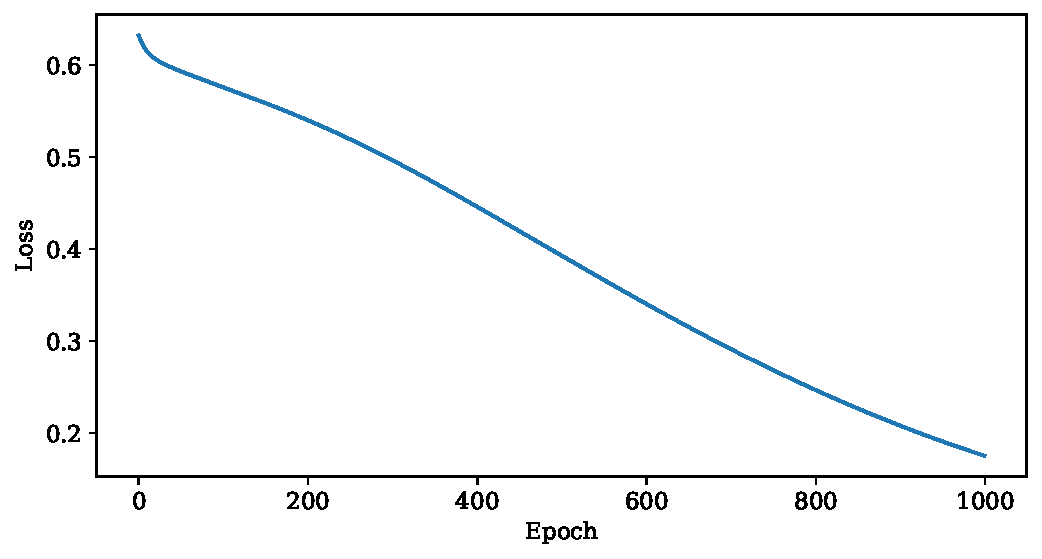
\includegraphics[width=\textwidth]{img/and_loss.pdf}
        \caption{AND function}
        \label{fig:and_loss}
    \end{subfigure}
    \hfill
    \begin{subfigure}[b]{0.48\textwidth}
        \centering
        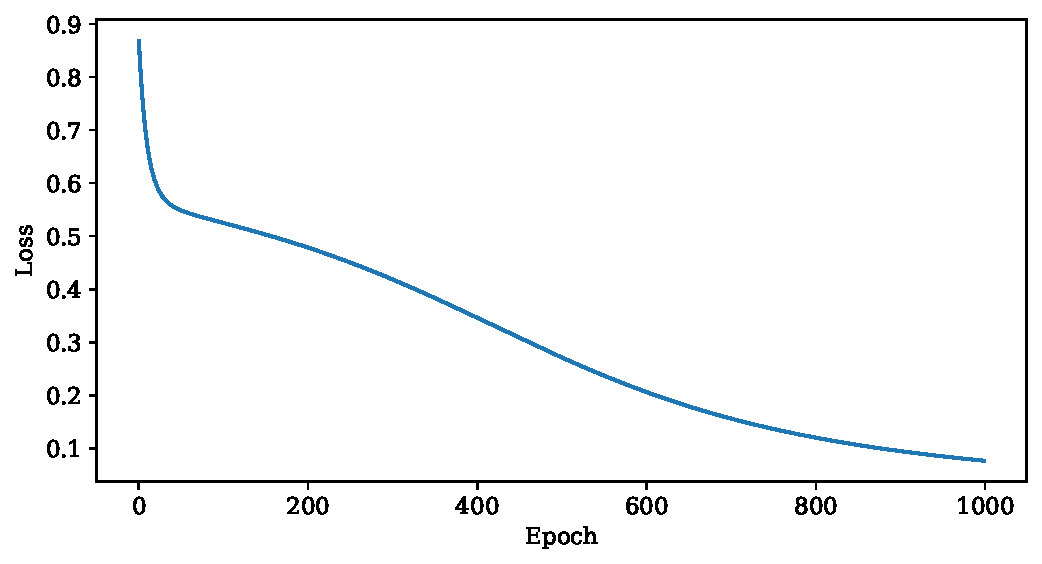
\includegraphics[width=\textwidth]{img/or_loss.pdf}
        \caption{OR function}
        \label{fig:or_loss}
    \end{subfigure}
    \vskip\baselineskip
    \begin{subfigure}[b]{0.48\textwidth}
        \centering
        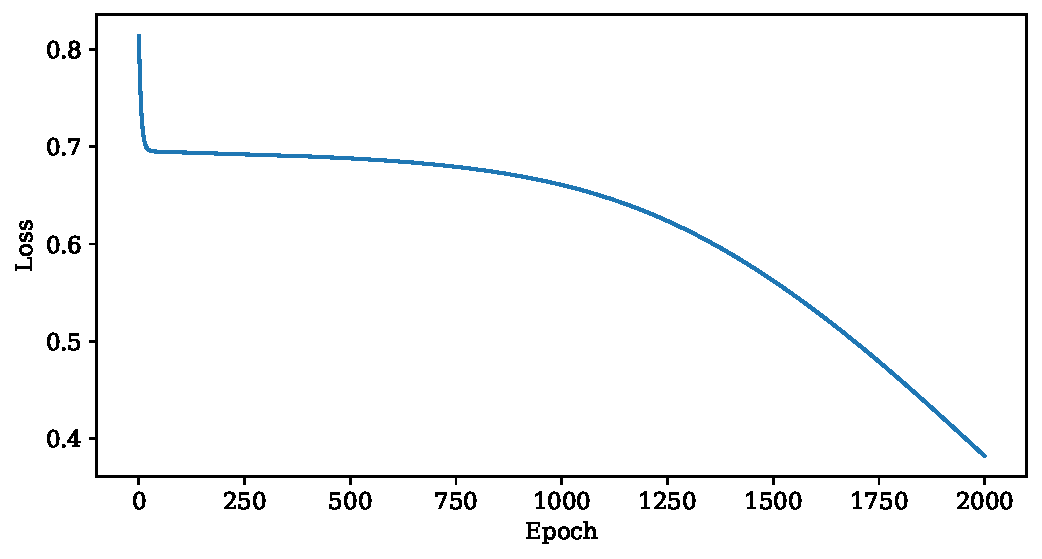
\includegraphics[width=\textwidth]{img/xor_loss.pdf}
        \caption{XOR function}
        \label{fig:xor_loss}
    \end{subfigure}
    \caption{Training loss curves for logical functions}
    \label{fig:loss_curves}
    \end{minipage}
    }
\end{figure}

\begin{figure}[H]
    \centering
    \fbox{
    \begin{minipage}{0.98\textwidth}
    \centering
    \begin{subfigure}[b]{0.48\textwidth}
        \centering
        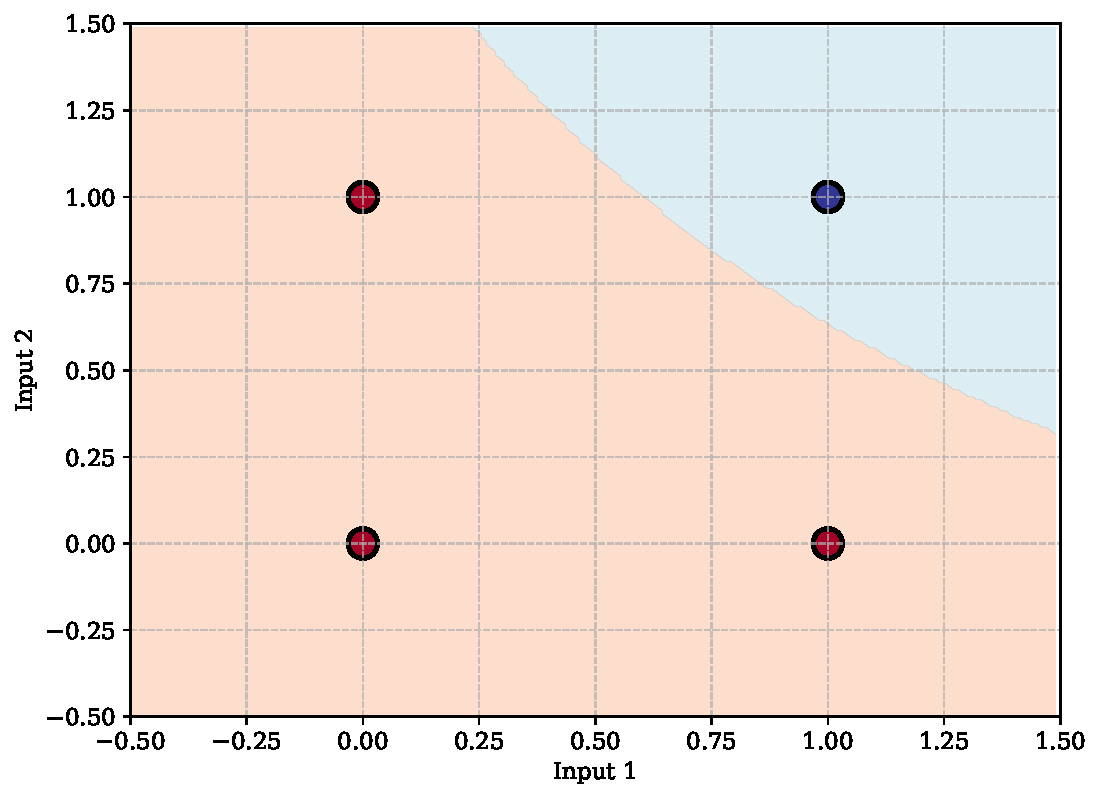
\includegraphics[width=\textwidth]{img/and_boundary.pdf}
        \caption{AND function}
        \label{fig:and_boundary}
    \end{subfigure}
    \hfill
    \begin{subfigure}[b]{0.48\textwidth}
        \centering
        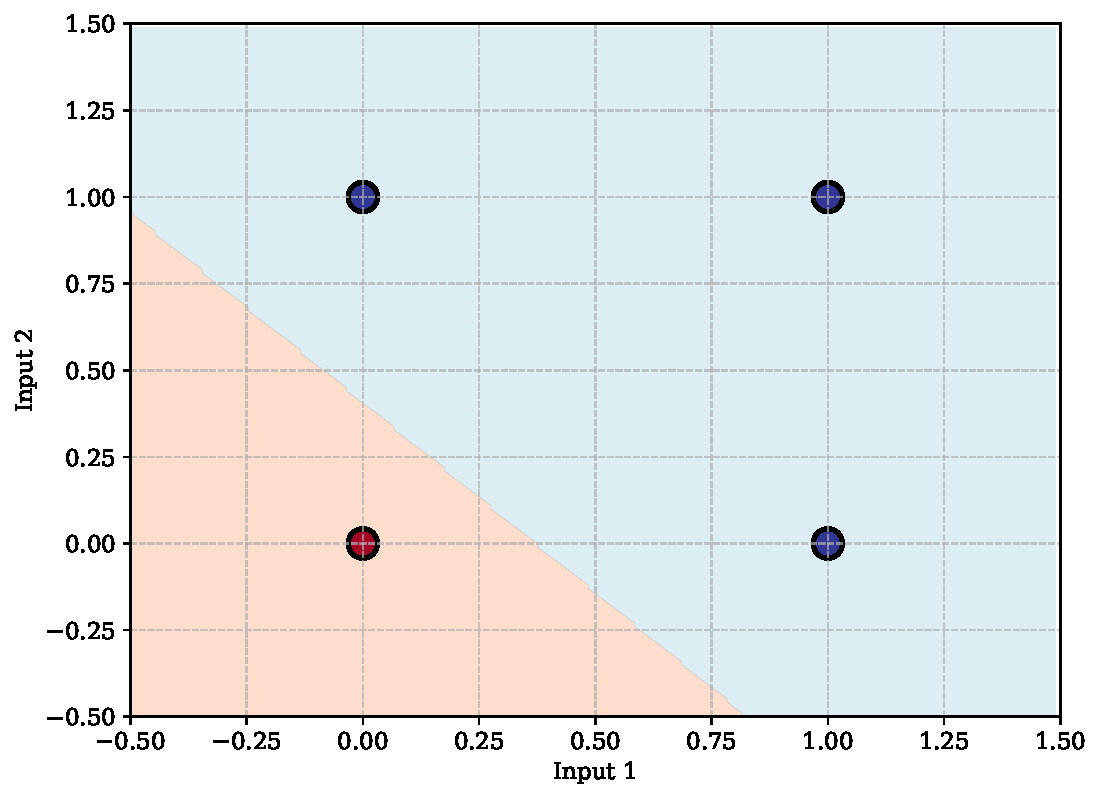
\includegraphics[width=\textwidth]{img/or_boundary.pdf}
        \caption{OR function}
        \label{fig:or_boundary}
    \end{subfigure}
    \vskip\baselineskip
    \begin{subfigure}[b]{0.48\textwidth}
        \centering
        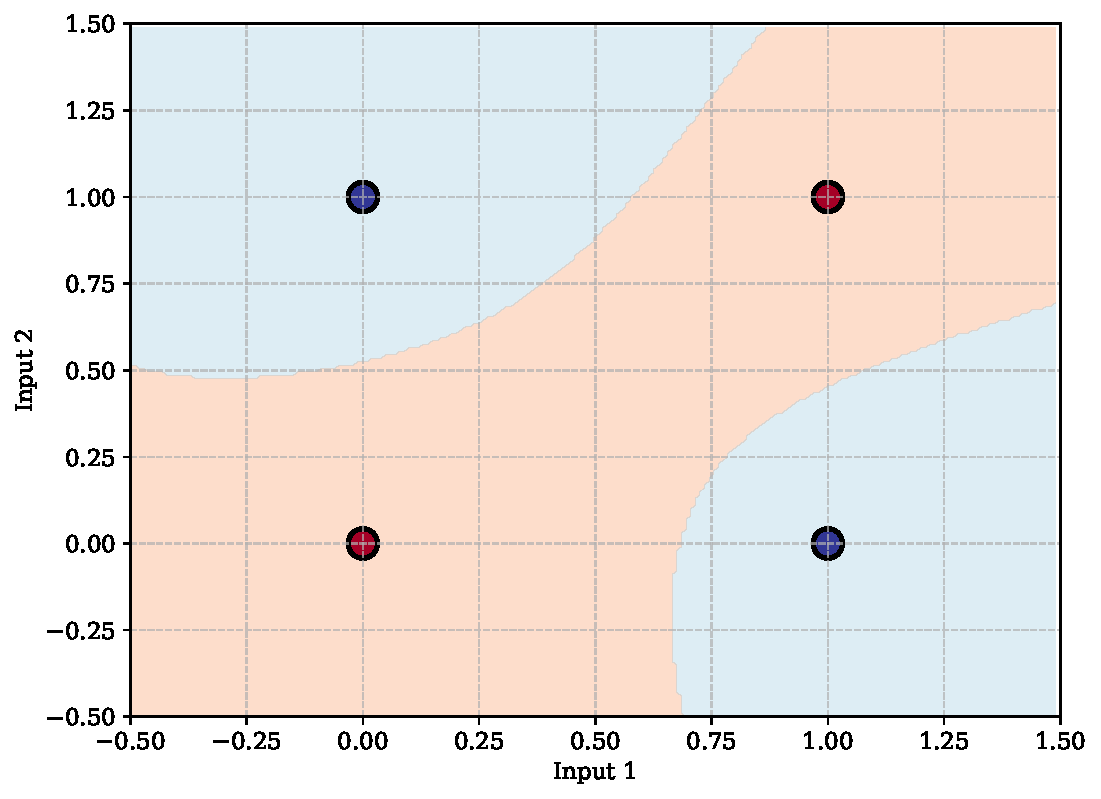
\includegraphics[width=\textwidth]{img/xor_boundary.pdf}
        \caption{XOR function}
        \label{fig:xor_boundary}
    \end{subfigure}
    \caption{Decision boundaries for logical functions}
    \label{fig:decision_boundaries}
    \end{minipage}
    }
\end{figure}

\begin{table}[H]
    \centering
    \caption{Predictions for AND function}
    \label{tab:and_pred}
    \csvautotabular{tab/and_predictions.csv}
\end{table}

\begin{table}[H]
    \centering
    \caption{Predictions for OR function}
    \label{tab:or_pred}
    \csvautotabular{tab/or_predictions.csv}
\end{table}

\begin{table}[H]
    \centering
    \caption{Predictions for XOR function}
    \label{tab:xor_pred}
    \csvautotabular{tab/xor_predictions.csv}
\end{table}

\section{Interpretation and Discussions}
\label{sec:discussion}
The network's ability to learn all three logical functions, particularly the XOR function, demonstrates the power of multi layer perceptrons in capturing both simple and complex relationships in the data.

The learning process reveals interesting patterns in how the network approaches different functions. For the simpler AND and OR functions, the network quickly converges to a solution, learning linear decision boundaries that effectively separate the classes. This rapid convergence is reflected in the training loss curves, which show steep initial decreases followed by stable performance. The prediction probabilities for these functions show high confidence in the correct classifications, with the OR function particularly showing very high confidence (0.95-0.99) in its true predictions.

The XOR function is a more challenging learning task, requiring the network to learn a non-linear decision boundary. This higher complexity is clear in several aspects of the results. The training loss curve shows a more gradual convergence, and the prediction probabilities are more balanced, with true cases predicted with probabilities around 0.80-0.82. This more moderate confidence level is due to the complexity of the XOR function and the network's need to learn a more difficult scenario.

Additionally, while the simpler AND and OR functions were learned effectively with 4 hidden units, the XOR function required 8 hidden units to achieve good performance. This relationship between function complexity and network capacity shows how important an appropriate architecture is in neural network design.

The decision boundary visualizations give a clear representation of how the network separates the input space for each function. The linear boundaries learned for AND and OR functions are optimal for these operations, while the non-linear boundary for XOR show once again that the network has learned a more complex relationship.

These results validate our implementation of backpropagation and demonstrate its effectiveness in learning both simple and complex logical functions. The network's ability to learn XOR shows that our implementation can capture non-linear relationships, which is important for more complex machine learning tasks.

\section{Conclusions}
\label{sec:conclusions}
This project demonstrates a from-scratch implementation of backpropagation for training multi-layer perceptrons and its application to learning basic logical functions. Our main findings include:

\begin{itemize}
\item The backpropagation implementation passed numerical gradient checking, ensuring the correctness of gradient computations.
\item The neural network successfully learned the AND, OR, and XOR functions, with loss curves and decision boundaries validating the learning process.
\item Linearly separable functions (AND, OR) were learned rapidly with shallow networks, while XOR required more hidden units and training time due to its non-linear nature.
\item Decision boundary visualizations show the non-linearity of the XOR model.
\end{itemize}

\section{Future Work}
\label{sec:future}
Several directions can extend the scope of this project:

\begin{itemize}
\item \textbf{Activation functions}: Incorporate other non-linearities such as ReLU or tanh to study their effects on training dynamics and convergence.
\item \textbf{Architecture scaling}: Extend the framework to support deeper or wider networks, including dropout and batch normalization layers.
\item \textbf{Real-world datasets}: Apply the backpropagation implementation to slightly more complex datasets such as MNIST or Iris to assess generalization and scalability.
\item \textbf{Visualization tools}: Create interactive tools for visualizing weight evolution and gradient flow.
\end{itemize}

\bibliographystyle{ieeetr}
\bibliography{references}

\end{document}
